\documentclass[preview,convert={convertexe={magick},outext=.ps}]{standalone}
\usepackage[dvipdfm]{geometry}
%graphics
\usepackage{xcolor}
\usepackage{tikz}
\usetikzlibrary{shapes.geometric, shapes.multipart, arrows, calc, through}
\usepackage[caption=false,font=footnotesize]{subfig}


\begin{document}

\begin{figure}[!t]
\centering
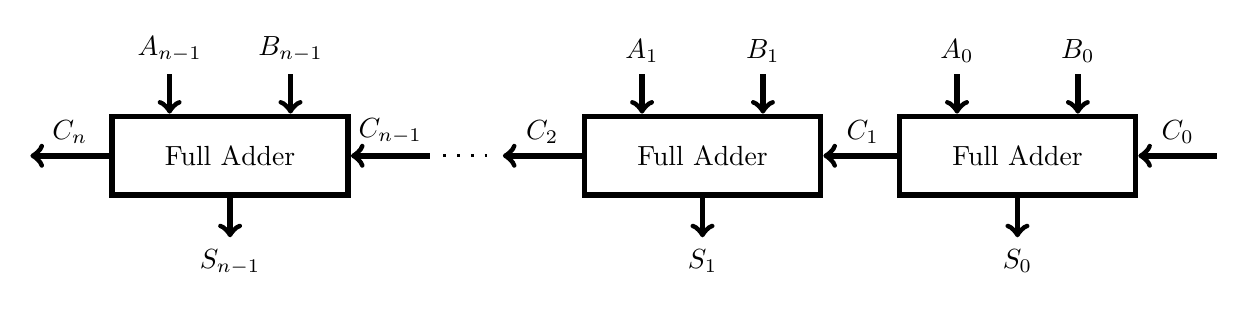
\begin{tikzpicture}

\node (A) [shape=rectangle,draw,line width=2pt,minimum width=3cm,minimum height=1cm] at (0,0) {Full Adder};
\draw[->,line width=2pt] ($(A.west)$) -- node[above]{$C_n$} ++(-1cm, 0);
\draw[<-,line width=2pt] ($(A.east)$) -- node[above]{$C_{n-1}$} ++(1cm, 0);
\draw[->,line width=2pt] ($(A.south)$) -- ++(0, -0.5cm) node[below]{$S_{n-1}$}; 
\draw[<-,line width=2pt] ($(A.north)!0.5!(A.north west)$) -- ++(0, 0.5cm) node[above]{$A_{n-1}$};
\draw[<-,line width=2pt] ($(A.north)!0.5!(A.north east)$) -- ++(0, 0.5cm) node[above]{$B_{n-1}$};

\node (A1) [shape=rectangle,draw,line width=2pt,minimum width=3cm,minimum height=1cm] at (6,0) {Full Adder};
\draw[->,line width=2pt] ($(A1.west)$) -- node[above]{$C_2$} ++(-1cm, 0);
\draw[<-,line width=2pt] ($(A1.east)$) -- node[above]{$C_1$} ++(1cm, 0);
\draw[->,line width=2pt] ($(A1.south)$) -- ++(0, -0.5cm) node[below]{$S_1$}; 
\draw[<-,line width=2pt] ($(A1.north)!0.5!(A1.north west)$) -- ++(0, 0.5cm) node[above]{$A_1$};
\draw[<-,line width=2pt] ($(A1.north)!0.5!(A1.north east)$) -- ++(0, 0.5cm) node[above]{$B_1$};

\node (A0) [shape=rectangle,draw,line width=2pt,minimum width=3cm,minimum height=1cm] at (10,0) {Full Adder};
\draw[<-,line width=2pt] ($(A0.east)$) -- node[above]{$C_0$} ++(1cm, 0);
\draw[->,line width=2pt] ($(A0.south)$) -- ++(0, -0.5cm) node[below]{$S_0$}; 
\draw[<-,line width=2pt] ($(A0.north)!0.5!(A0.north west)$) -- ++(0, 0.5cm) node[above]{$A_0$};
\draw[<-,line width=2pt] ($(A0.north)!0.5!(A0.north east)$) -- ++(0, 0.5cm) node[above]{$B_0$};

\draw[loosely dotted, line width=1pt] ($(A.east)!.4!(A1.west)$) -- ($(A.east)!.6!(A1.west)$);

\end{tikzpicture}
\end{figure}

\end{document}
